\section{Логические алгоритмы. Решающие деревья}

\subsection{Введение}

Логическая закономерность в задачах классификации — легко интерпретируемое правило, выделяющее из обучающей выборки достаточно много объектов какого-то одного класса и практически не выделяющее объекты остальных классов. Логические закономерности являются элементарными «строительными блоками» для широкого класса логических алгоритмов классификации, называемых также алгоритмами индукции правил 

В логических алгоритмах классификации принцип в индуктивном выводе логических закономерностей или индукции правил. Пусть $\phi:X \implies {0;1}$ — некоторый предикат, определённый на множестве объектов $X$. Говорят, что предикат $\phi$ выделяет или покрывает объект $x$, если $\phi(x) = 1$. Предикат называют закономерностью, если он выделяет достаточно много объектов какого-то одного класса $c$, и практически не выделяет объекты других классов. 

Особую ценность представляют закономерности, которые описываются простой логической формулой. Их называют правилами (rules). Процесс поиска правил по выборке называют извлечением знаний из данных. К знаниям предъявляется особое требование — они должны быть интерпретируемы, то есть понятны людям. На практике логические закономерности часто ищут в виде конъюнкций небольшого числа элементарных высказываний. Именно в такой форме люди привыкли выражать свой житейский и профессиональный опыт.

Всякая закономерность классифицирует лишь некоторую часть объектов. Объединив определённое количество закономерностей в композицию, можно получить алгоритм, способный классифицировать любые объекты. Логическими алгоритмами классификации будем называть композиции легко интерпретируемых закономерностей. 

Общая задача звучит так:
Имеется пространство объектов $X$ и конечное множество имён классов $Y= {1,...,M}$. Целевая зависимость $y^{*}: X \implies Y$ известа только на объектах обучающей выборки $X_l=(x_i,y_i)$.  Требуется построить алгоритм классификации $\alpha: X \implies Y$, аппроксимирующий $y^{*}$ на всё множестве $X$.

\subsection{Информативность}

Эвристическое определение информативности. Интуитивно предикат $\phi$ тем более информативен, чем больше он покрывает объектов некоторого фиксированного «своего» класса сY по сравнению с объектами всех остальных «чужих» классов. Введём следующие обозначения:
$G_c$ - число объектов класса с в выборке $X_l$
$g_c(\phi)$ - из них число объектов, для которых выполняется условие $(\phi(х) = 1)$
$B_c$ - число объектов всех остальных классов $Y \setminus {c}$ в выборке $X_l$
$b_c(\phi)$ -  из них число объектов, для которых выполняется условие $\phi(х) = 1$.

Чем   больше   число   покрываемых объектов $(g+b)$ и чем меньше среди них ошибочных $b$, тем более информативен предикат $\phi$. И, наоборот, наименее интересны предикаты, которые либо покрывают слишком мало объектов, либо выделяют «свои» и «чужие» объекты примерно в той же пропорции, в которой они представлены во всей выборке, $b:g \sim B:G$.

Введём обозначение $E_c$ для доли ошибочно покрываемых «чужих» объектов, и $D_c$ для доли всех покрываемых объектов:

\begin{subequations}
\begin{align}
	E_c(\phi,X_l)=\frac{b_c(\phi)}{b_c(\phi)+g_c(\phi)} \\
	D_c(\phi,X_l)=\frac{b_c(\phi)+g_x(\phi)}{l}
\end{align}
\end{subequations}

Если $bс(\phi)=0$, то закономерность $\phi$ называется чистой или непротиворечивой.Если $b_c(\phi)>0$, то закономерность $\phi$ называется частичной.

В некоторых случаях имеет смысл ограничиваться поиском только чистых закономерностей. В частности, когда длина выборки мала или заранее известно, что данные практически не содержат шума. Такие прикладные задачи нередко встречаются на практике, например, классификация месторождений редких полезных ископаемых по данным геологоразведки.

Но чаще данные оказываются неполными и неточными. Таковы многие медицинские и экономические задачи (в частности, задача о выдаче кредитов). Для них незначительная доля ошибок $\epsilon$ на обучающей выборке вполне допустима. Кроме того, существуют способы построения корректных алгоритмов на основе частичных закономерностей, например, взвешенное голосование. В этих случаях сравнивать и отбирать предикаты приходится по двум критериям $(g,b)$ одновременно.

\subsection{Информационная энтропия}

Информационная энтропия — мера неопределённости или непредсказуемости информации, неопределённость появления какого-либо символа первичного алфавита. При отсутствии информационных потерь численно равна количеству информации на символ передаваемого сообщения.

Например, в последовательности букв, составляющих какое-либо предложение на русском языке, разные буквы появляются с разной частотой, поэтому неопределённость появления для некоторых букв меньше, чем для других. Если же учесть, что некоторые сочетания букв (в этом случае говорят об энтропии n-ого порядка, см. ниже) встречаются очень редко, то неопределённость уменьшается еще сильнее.

Для иллюстрации понятия информационной энтропии можно также прибегнуть к примеру из области термодинамической энтропии, получившему название демона Максвелла. Концепции информации и энтропии имеют глубокие связи друг с другом, но, несмотря на это, разработка теорий в статистической механике и теории информации заняла много лет, чтобы сделать их соответствующими друг другу.

Энтропия — это количество информации, приходящейся на одно элементарное сообщение источника, вырабатывающего статистически независимые сообщения.

Энтропийное определение информативности. Ещё один способ определения информативности вытекает из теории информации. Если имеются два исхода $w_0$ , $w_1$ с вероятностями $q_0$ и $q_1=1-q_0$, то количество информации, связанное с исходом $w_i$ , по определению равно $-\log_2 q_i$. Это математическое ожидание числа бит, необходимых для записи информации о реализации исходов $w_i$ при использовании оптимального (наиболее экономного) кодирования. Энтропия определяется как матожидание количества информации:

\begin{equation}
	H(q_0,q_1)=-q_0\log_2 q_0-q_1\log_2 q_1
\end{equation}

Будем считать появление объекта класса $c$ исходом $w_0$, а появление объекта любого другого класса исходом $w_1$. Тогда, подставляя вместо вероятностей частоты, можно оценить энтропию выборки $X_l$:

\begin{equation}
	H(P,N)=H(\frac{P}{P+N},\frac{N}{N+P})
\end{equation}

Допустим, стало известно, что предикат $\phi$ выделил $p$ объектов из $P$, принад-
лежащих классу $c$, и $n$ объектов из $N$, не принадлежащих классу $c$. Тогда энтропия выборки ${x\in X_l|\phi(x)=1}$ есть $H(p,n)$. Вероятность появления объекта из этой выборки оценивается как $\frac{p+n}{P+N}$. Аналогично, энтропия выборки ${x\in X_l|\phi(x)=0}$ есть $H(P-p,N-n)$, а вероятность появления объекта из неё оценивается как $\frac{P-p+N-n}{P+N}$. Таким образом, энтропия всей выборки после получения информации $\phi$ становится равна

\begin{equation}
	H_{\phi}(P,N,p,n)=\frac{p+n}{P+N}H(p,n) + \frac{P+N-p-n}{P+N}H(P-p,N-n)
\end{equation}

В итоге уменьшение энтропии составит:

\begin{equation}
	{IGain}_c(\phi,X_l)=H(P,N)-H(P,N,p,n)
\end{equation}

Это и есть информационный выигрыш (information gain) — количество информа-
ции об исходном делении выборки на два класса $c$ и $не c$, которое содержится
в предикате $\phi$. Таким образом, появляется ещё одно, альтернативное, определение
закономерности.

Несмотря на асимптотическую эквивалентность, значения $I_c$ и ${IGain}_c$ могут заметно отличаться при малых $n$ или $p$. Согласно таблице 1, критерий ${IGain}_c$ полагает, что «маломощная» закономерность $(n,p)=(0,5)$ лучше, чем «полное отсутствие закономерности» $(50,100)$, тогда как точный тест $I_c$ показывает противоположное. Иными словами, критерий IGain завышает информативность маломощных закономерностей. Ситуации малых $n$ или $p$ вовсе не экзотичны, они регулярно возникают при построении решающих списков и деревьев. Точный критерий может давать в этих ситуациях ощутимые преимущества ~\cite{martin}. Однако на практике чаще используется энтропийный критерий, поскольку он проще вычисляется.

Когда число классов превышает 3, приходится оценивать информативность не только таких предикатов, которые отделяют один класс от остальных, но и таких, которые отделяют некоторую группу классов от остальных.

Энтропийный критерий для случая большого числа классов:

\begin{equation}
	I(\phi,X_l)=\sum_{c\in Y}h(\frac{P_c}{l})-\frac{p}{l}\sum_{c\in Y}h(\frac{p_c}{p})-\frac{l-p}{l}\sum_{c\in Y}h(\frac{P_c-p_c}{l-p})
\end{equation}
где введена функция $h(z)=-z\log_2 z$.

\subsection{Решающие деревья.}

Решающее дерево — это логический алгоритм классификации, основанный на поиске конъюнктивных закономерностей. При синтезе дерева все конъюнкции строятся одновременно. Деревом называется конечный связный граф с множеством вершин $V$ , не содержащий циклов и имеющий выделенную вершину $v_0 \in V$ , в которую не входит ни одно ребро. Эта вершина называется корнем дерева. Вершина, не имеющая выходящих рёбер, называется терминальной или листом. Остальные вершины называются внутренними. Дерево называется бинарным, если из любой его внутренней вершины выходит ровно два ребра. Выходящие рёбра связывают каждую внутреннюю вершину $v$ с левой дочерней вершиной $L_v$ и $с$ правой дочерней вершиной $R_v$.

Деревья классификации - это метод, позволяющий предсказывать принадлежность наблюдений или объектов к тому или иному классу категориальной зависимой переменной в зависимости от соответствующих значений одной или нескольких предикторных переменных. Построение деревьев классификации - один из наиболее важных методов, используемых при проведении добычи данных.

Цель построения деревьев классификации заключается в предсказании (или объяснении) значений категориальной зависимой переменной, и поэтому используемые методы тесно связаны с более традиционными методами Дискриминантного анализа, Кластерного анализа, Непараметрической статистики и Нелинейного оценивания. Широкая сфера применимости деревьев классификации делает их весьма привлекательным инструментом анализа данных.

\subsubsection{Детали реализации}

В данном дипломном проекте были использованы классифицирующие деревья решений~\cite{cart_book}. Дальше будет описан алгоритм построения таких деревьев для задачи ранжирования.

Для поиска атрибутов с максимальной информативностью была использована энтропия. Сам алгоритм разрабатывался с целью использования как слабого классифицирующего алгоритма в градиентном бустинге.

\begin{figure}
  \centering
  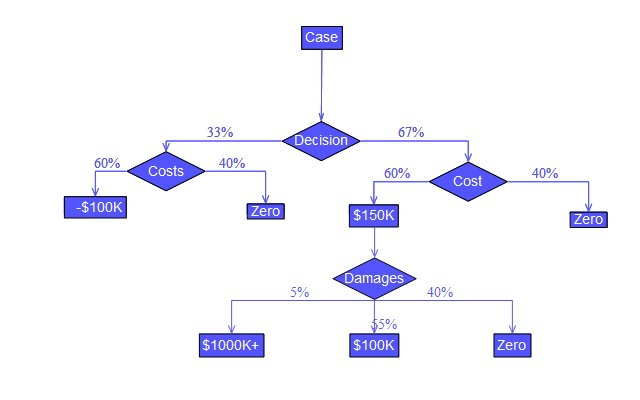
\includegraphics[width=1.0\textwidth]{images/Decision_tree_using_flow_chart_symbols.jpg}
  \caption{Пример решающего дерева\label{decision_tree_schema}}
\end{figure}

Структурна схема алгоритма приведена на рисунке ~\ref{decision_tree_schema}.

Сам алгоритм приведен на ~\ref{decision-tree-algorithm}:

\begin{algorithm}
  \caption{Алгоритм построения решающего дерева}
  \label{decision-tree-algorithm}
  \begin{enumerate}
  \item Загрузить обучающую выборку $(x_i,y_i)$
  \item Задать переменные $max_tree_depth,min_subset_length$
  \item Пока выполняется критерий
  	\begin{enumerate}
  		\item Выбрать атрибут из вектора $x_i$
  		\item Посчитать энтропию $H(Y)$
  		\item для каждого элемента обучающей выборки
  		\begin{enumerate}
  			\item Посчитать энтропию атрибута при $H(Y|X_i)$
  		\end{enumerate}
  		\item Взять атрибут $x_{ij}$ с максимальной информативностью.
  		\item Поделить выборку на 2.
  			\begin{subequations}
  			\begin{align}
  				R_1(j,s)={X|X_j < s} \\
  				R_2(j,s)={X|X_j > s}
  			\end{align}
  			\end{subequations}
  	\end{enumerate}
  \end{enumerate}
\end{algorithm}


Преимущества алгоритма:

\begin{itemize}
  \item Простота и интерпретируемость классификации. Алгоритм способен
не только классифицировать объект, но и выдать объяснение классификации
в терминах предметной области. Объяснение строится путём выписывания по-
следовательности условий, проверенных для данного объекта на пути от корня
дерева до листа $v$. Эти условия образуют конъюнкцию $K_v$ , то есть легко интер-
претируемое логическое правило.
  \item Не бывает отказов от классификации, в отличие от решающих списков.
  \item  Алгоритм очень прост для реализации и легко поддаётся различным усовершенствованиям. Можно использовать различные критерии ветвления и критерии останова, вводить редукцию, и т. д.
 \end{itemize}

Недостатки алгоритма:

\begin{itemize}
  \item Проблема получения оптимального дерева решений является NP-полной с точки зрения некоторых аспектов оптимальности даже для простых задач ~\cite{cart_optimal1} ~\cite{cart_optimal2}. Таким образом, практическое применение алгоритма деревьев решений основано на эвристических алгоритмах, таких как алгоритм «жадности», где единственно оптимальное решение выбирается локально в каждом узле. Такие алгоритмы не могут обеспечить оптимальность всего дерева в целом.
  \item Те, кто изучает метод дерева принятия решений, могут создавать слишком сложные конструкции, которые не достаточно полно представляют данные. Данная проблема называется проблемой «чрезмерной подгонки»~\cite{cart_optimal3} Для того, чтобы избежать данной проблемы, необходимо использовать Метод «регулирования глубины дерева».
  \item Существуют концепты, которые сложно понять из модели, так как модель описывает их сложным путем. Данное явление может быть вызвано проблемами XOR, четности или мультиплексарности. В этом случае мы имеем дело с непомерно большими деревьями. Существует несколько подходов решения данной проблемы, например, попытка изменить репрезентацию концепта в модели (составление новых суждений)~\cite{cart_optimal4}, или использование алгоритмов, которые более полно описывают и репрезентируют концепт (например, метод статистических отношений, индуктивная логика программирования).
  \item Для данных, которые включают категориальные переменные с большим набором уровней (закрытий), больший информационный вес присваивается тем атрибутам, которые имеют большее количество уровней.~\cite{cart_optimal5}
 \end{itemize}

В ходе разработки алгоритма, был построен алгоритм для решения задачи классификации с множеством классов. Т.к. данный алгоритм планируется использовать с градиентным бустингом, то редукция деревьев не была нужна. Максимальная глубина дерева составила 8. Кроме этого, все параметры вектора $x_i \in R$, поэтому при поиске наилушего атрибута приходилось пробегать по значению $x_{ij}$ для всей выборке. 